\documentclass[a4paper]{scrartcl}

\usepackage[utf8]{inputenc}
\usepackage[dutch]{babel}
\usepackage{a4wide}
\usepackage{graphicx}

\title{\#metoo}
\subtitle{}
\author{Casper van Velzen\\Rick van Bork\\Jelle den Haan\\Sebastiaan Arendsen}
\pagestyle{empty}

\begin{document}
\maketitle
\thispagestyle{empty}
\begin{figure}[h!]
    \begin{center}
        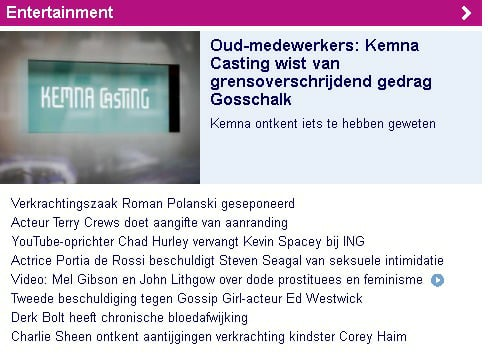
\includegraphics[scale=0.4]{nu.jpg}
    \end{center}
    \caption{75\% van het entertainmentnieuws.}
\end{figure}
De laatste tijd is er veel ophef in de media over seksuele intimidatie, vooral in de entertainment industrie.
\begin{itemize}
    \item Is er sprake van een toename in het aantal zaken?
        \begin{itemize}
            \item Is er verschil tussen verschillende mediabronnen?
            \begin{itemize}
                \item Visualisatie
            \end{itemize}
        \end{itemize}
    \item Is er verschil te zien in berichtgeving over deze zaken?
    \begin{itemize}
        \item Welke sleutelwoorden worden er gebruikt in de berichten?
            \begin{itemize}
                \item Visualisatie
            \end{itemize}
    \end{itemize}
\end{itemize}
\end{document}